We have designed five different PID controllers for each Gx, Gy, Gz and Ny outputs. We have created an individual closed loop system in order to check the response of the outputs with a PID controller. The closed loop system for Gx can be seen in Figure \ref{closedloop1}. The step Gxref represents the reference value of the output Gx. Both will be fed to the comparator and th PID controller will take care of the error.

\begin{figure}[H]
  \centering
    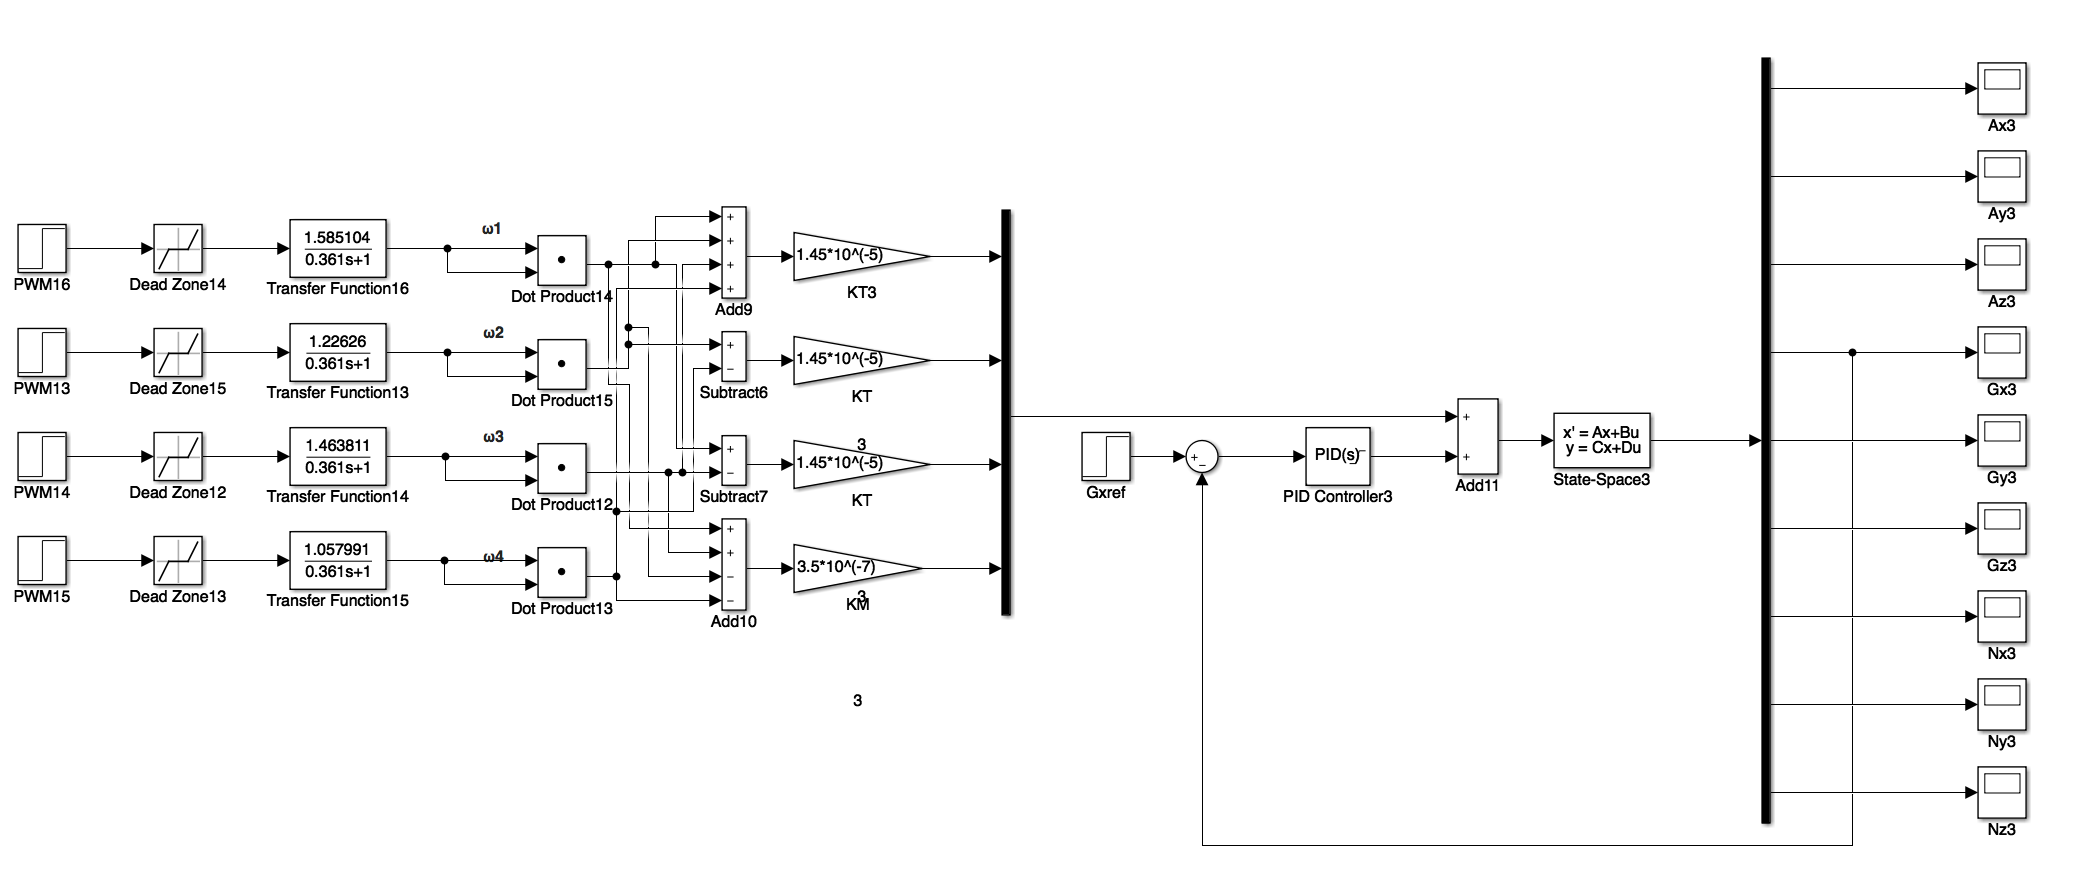
\includegraphics[width=1\textwidth]{images/closedloopGx.png}
	\caption{smth.}
	\label{closedloop1}
\end{figure}

The autotuning within the Simulink environment was used and the results are presented in Figures \ref{closedloop2} - \ref{closedloop5}.

\begin{figure}[H]
  \centering
    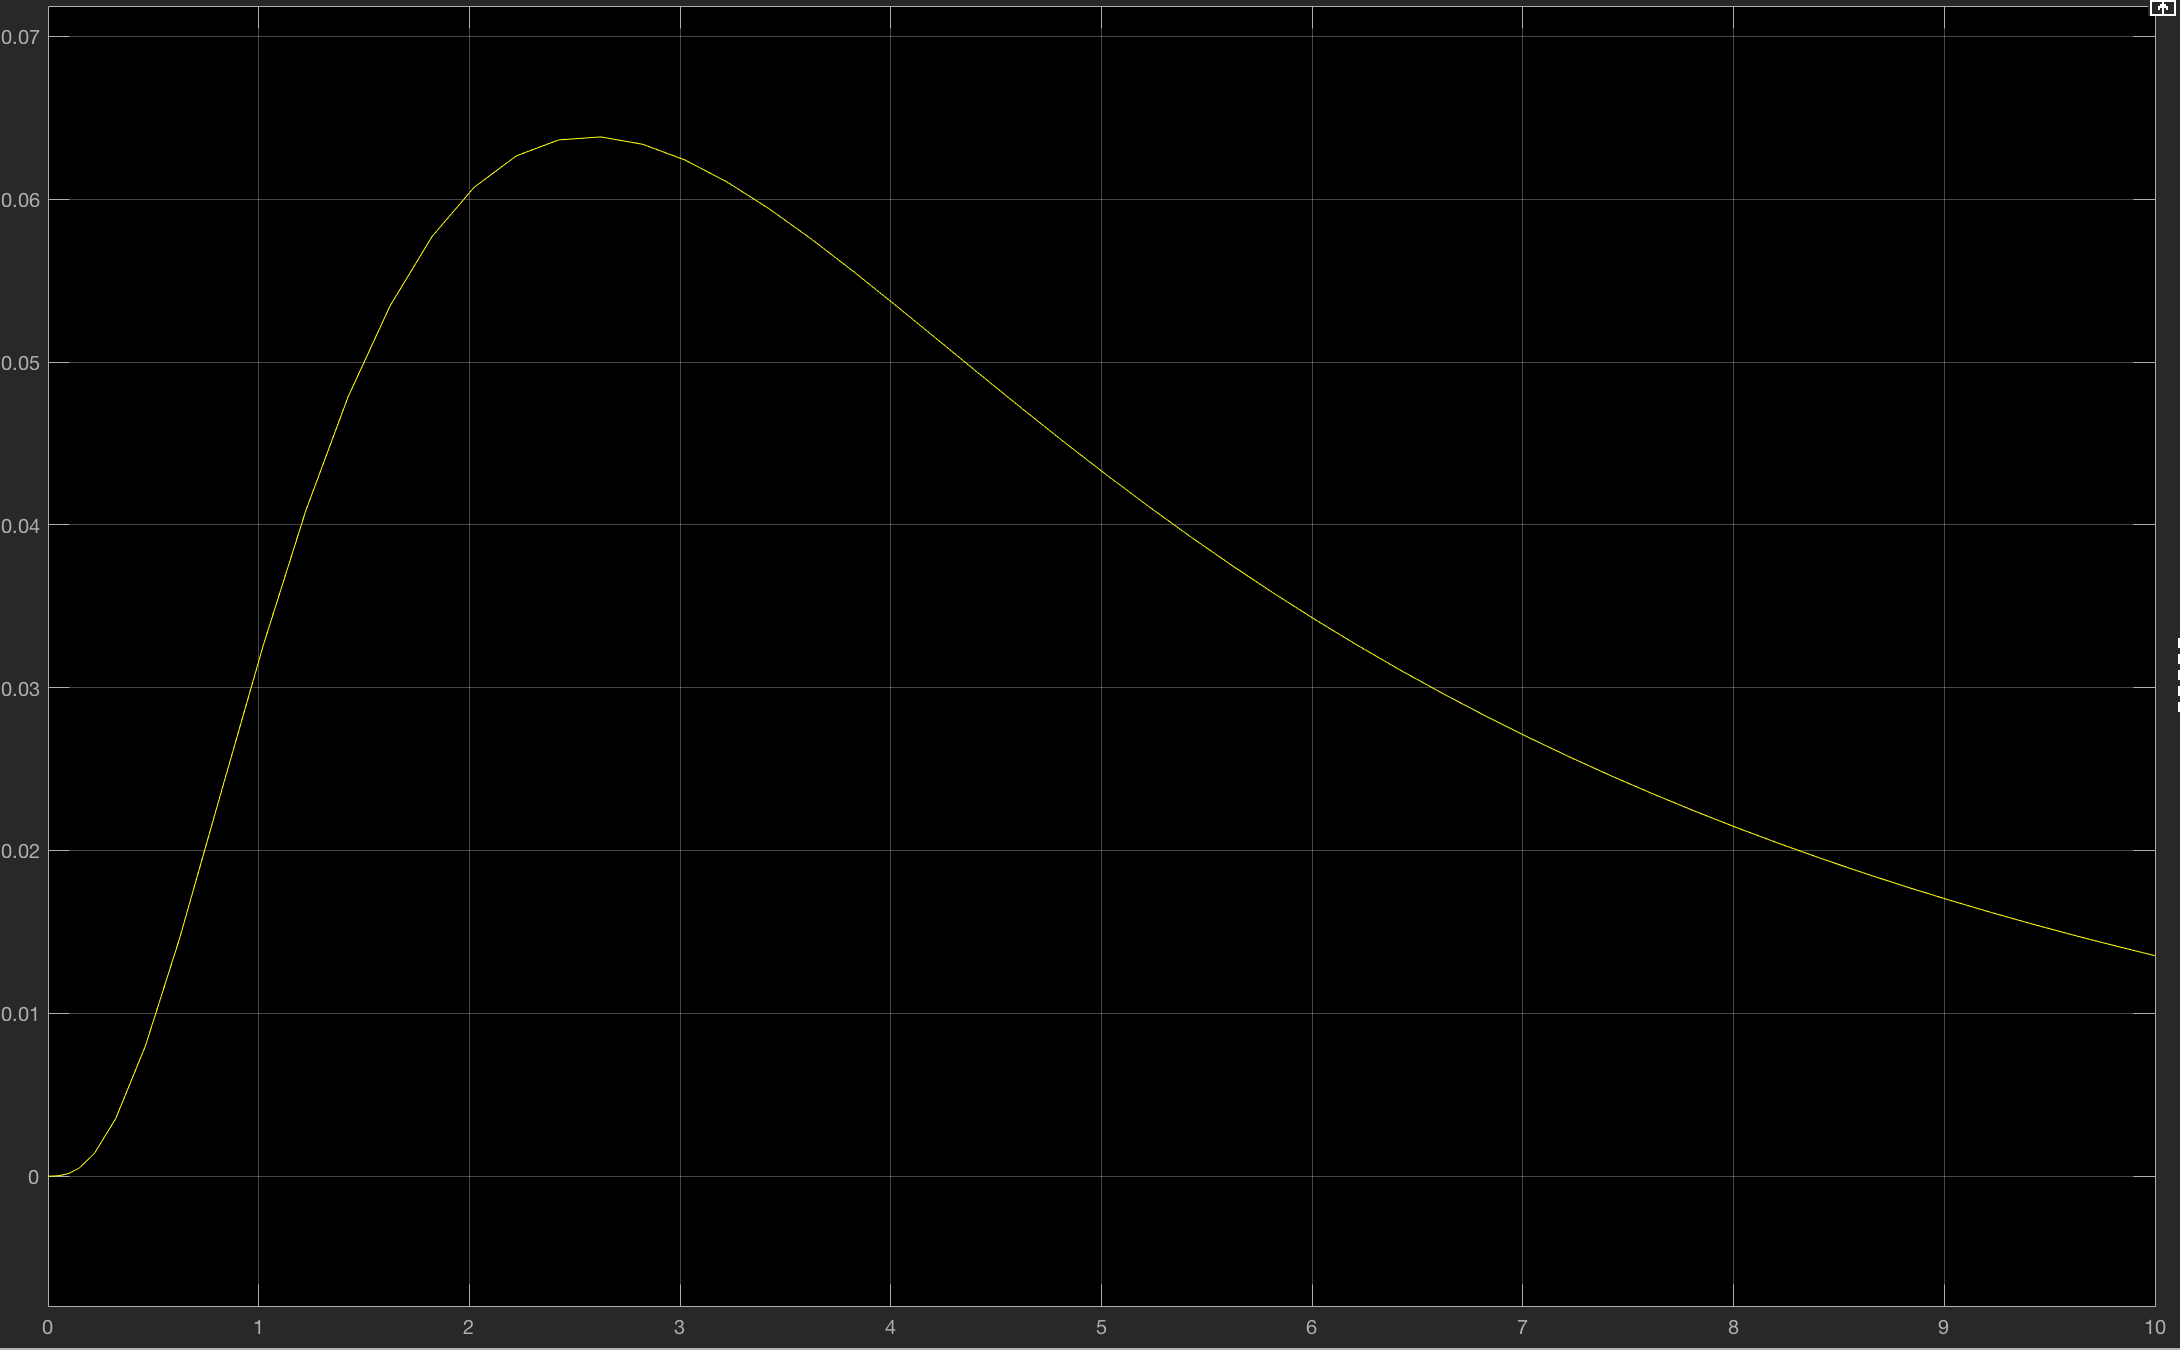
\includegraphics[width=1\textwidth]{images/closedloopGxstep.png}
	\caption{Closed loop response of the Gx output.}
	\label{closedloop2}
\end{figure}

\begin{figure}[H]
  \centering
    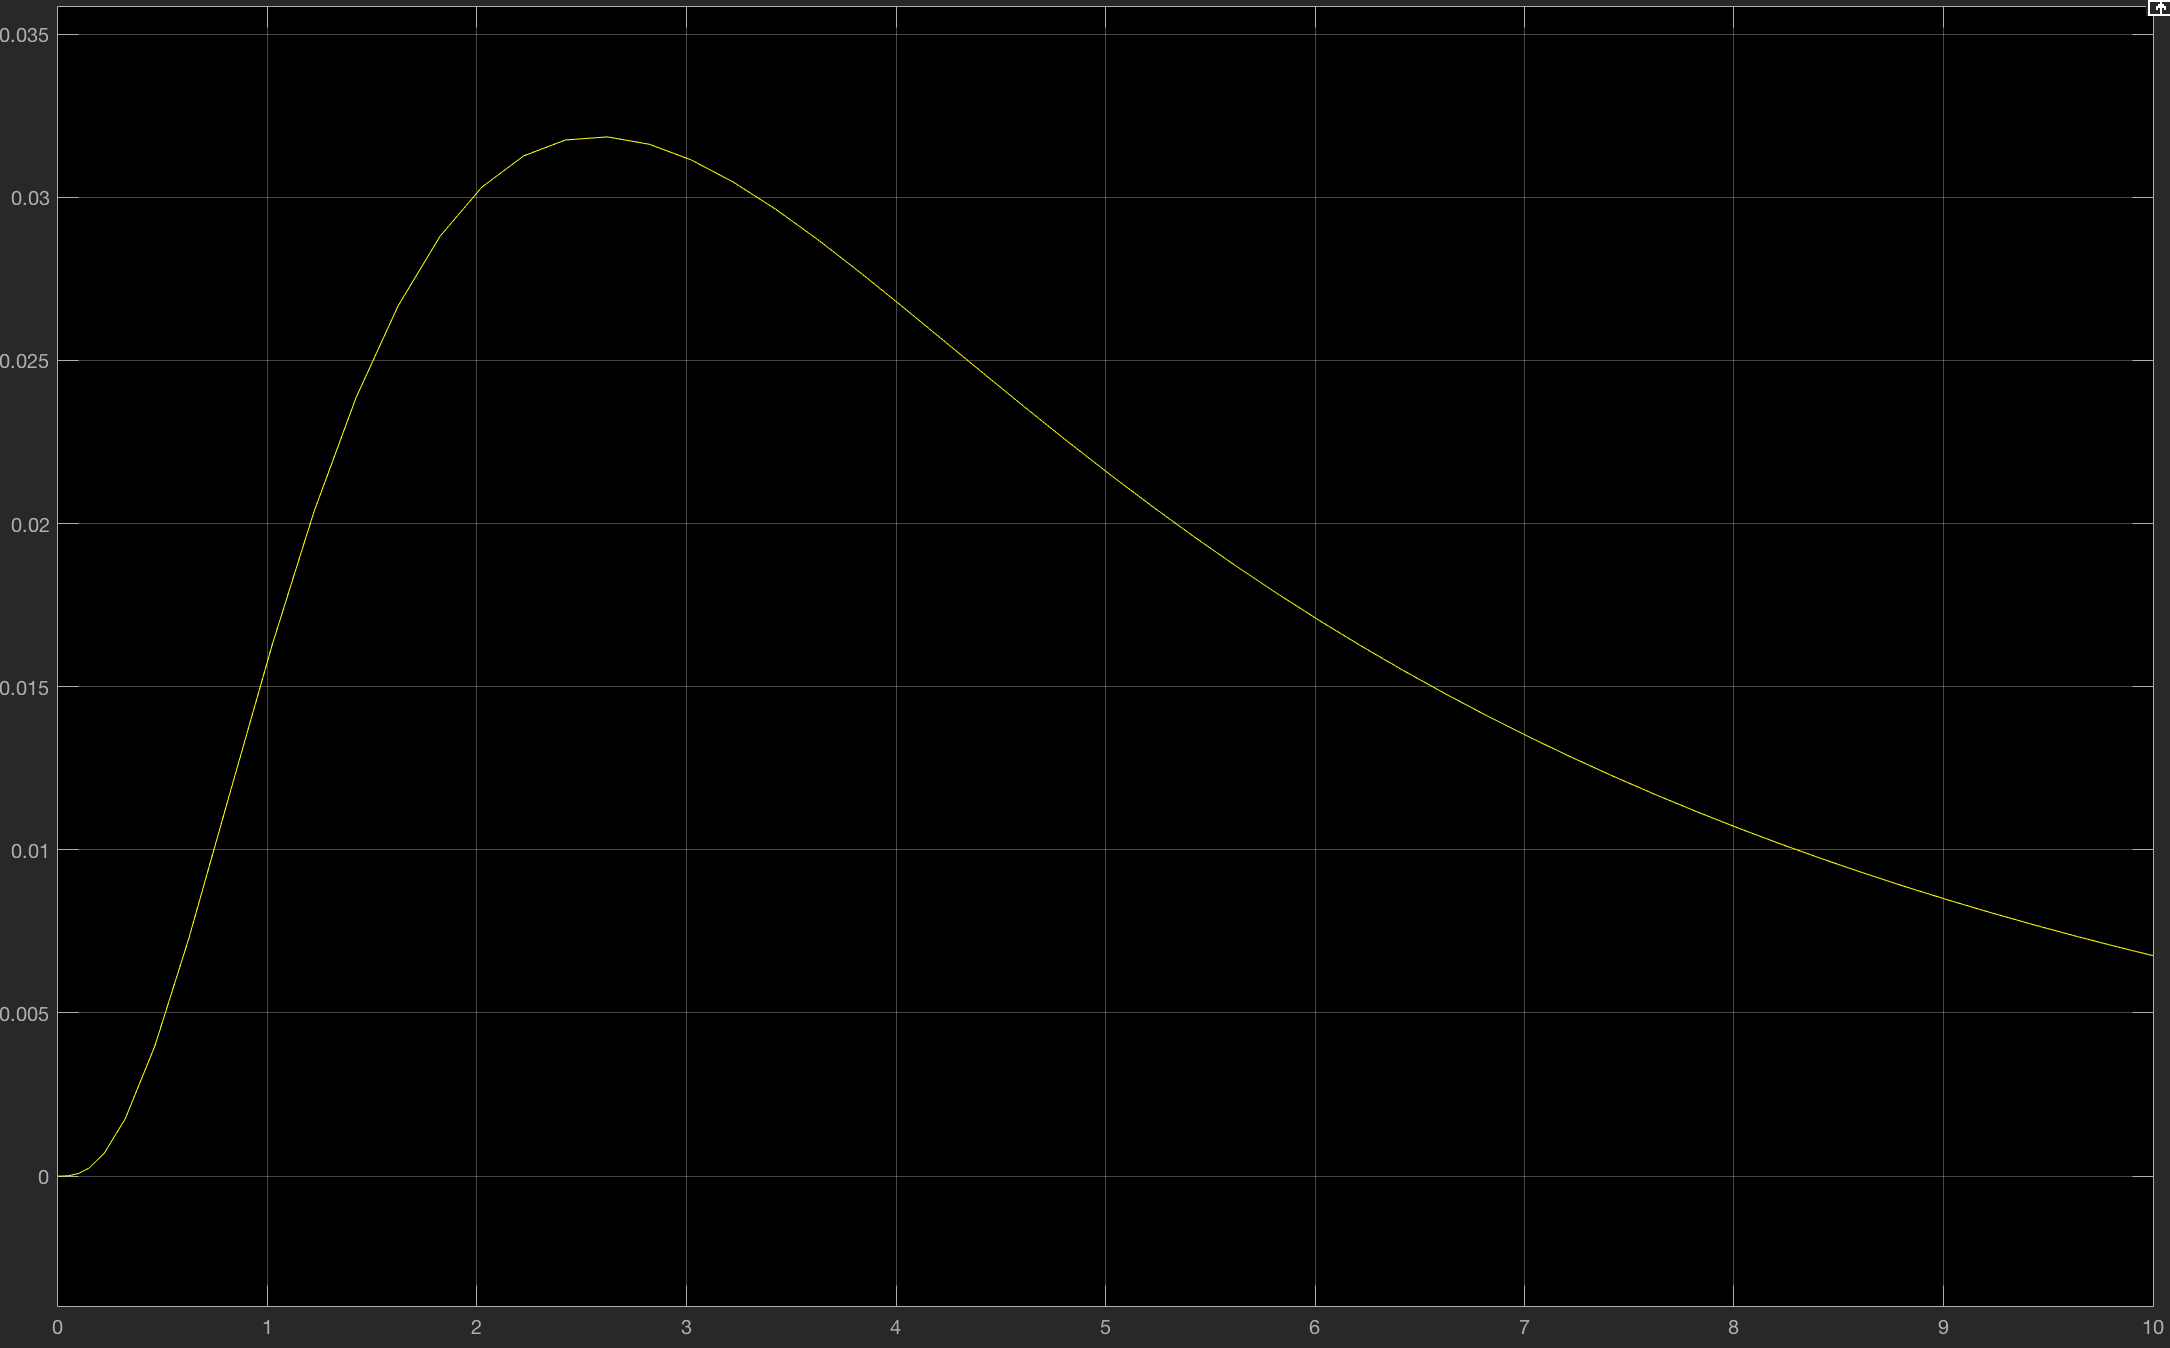
\includegraphics[width=1\textwidth]{images/closedloopGystep.png}
	\caption{Closed loop response of the Gy output.}
	\label{closedloop3}
\end{figure}

\begin{figure}[H]
  \centering
    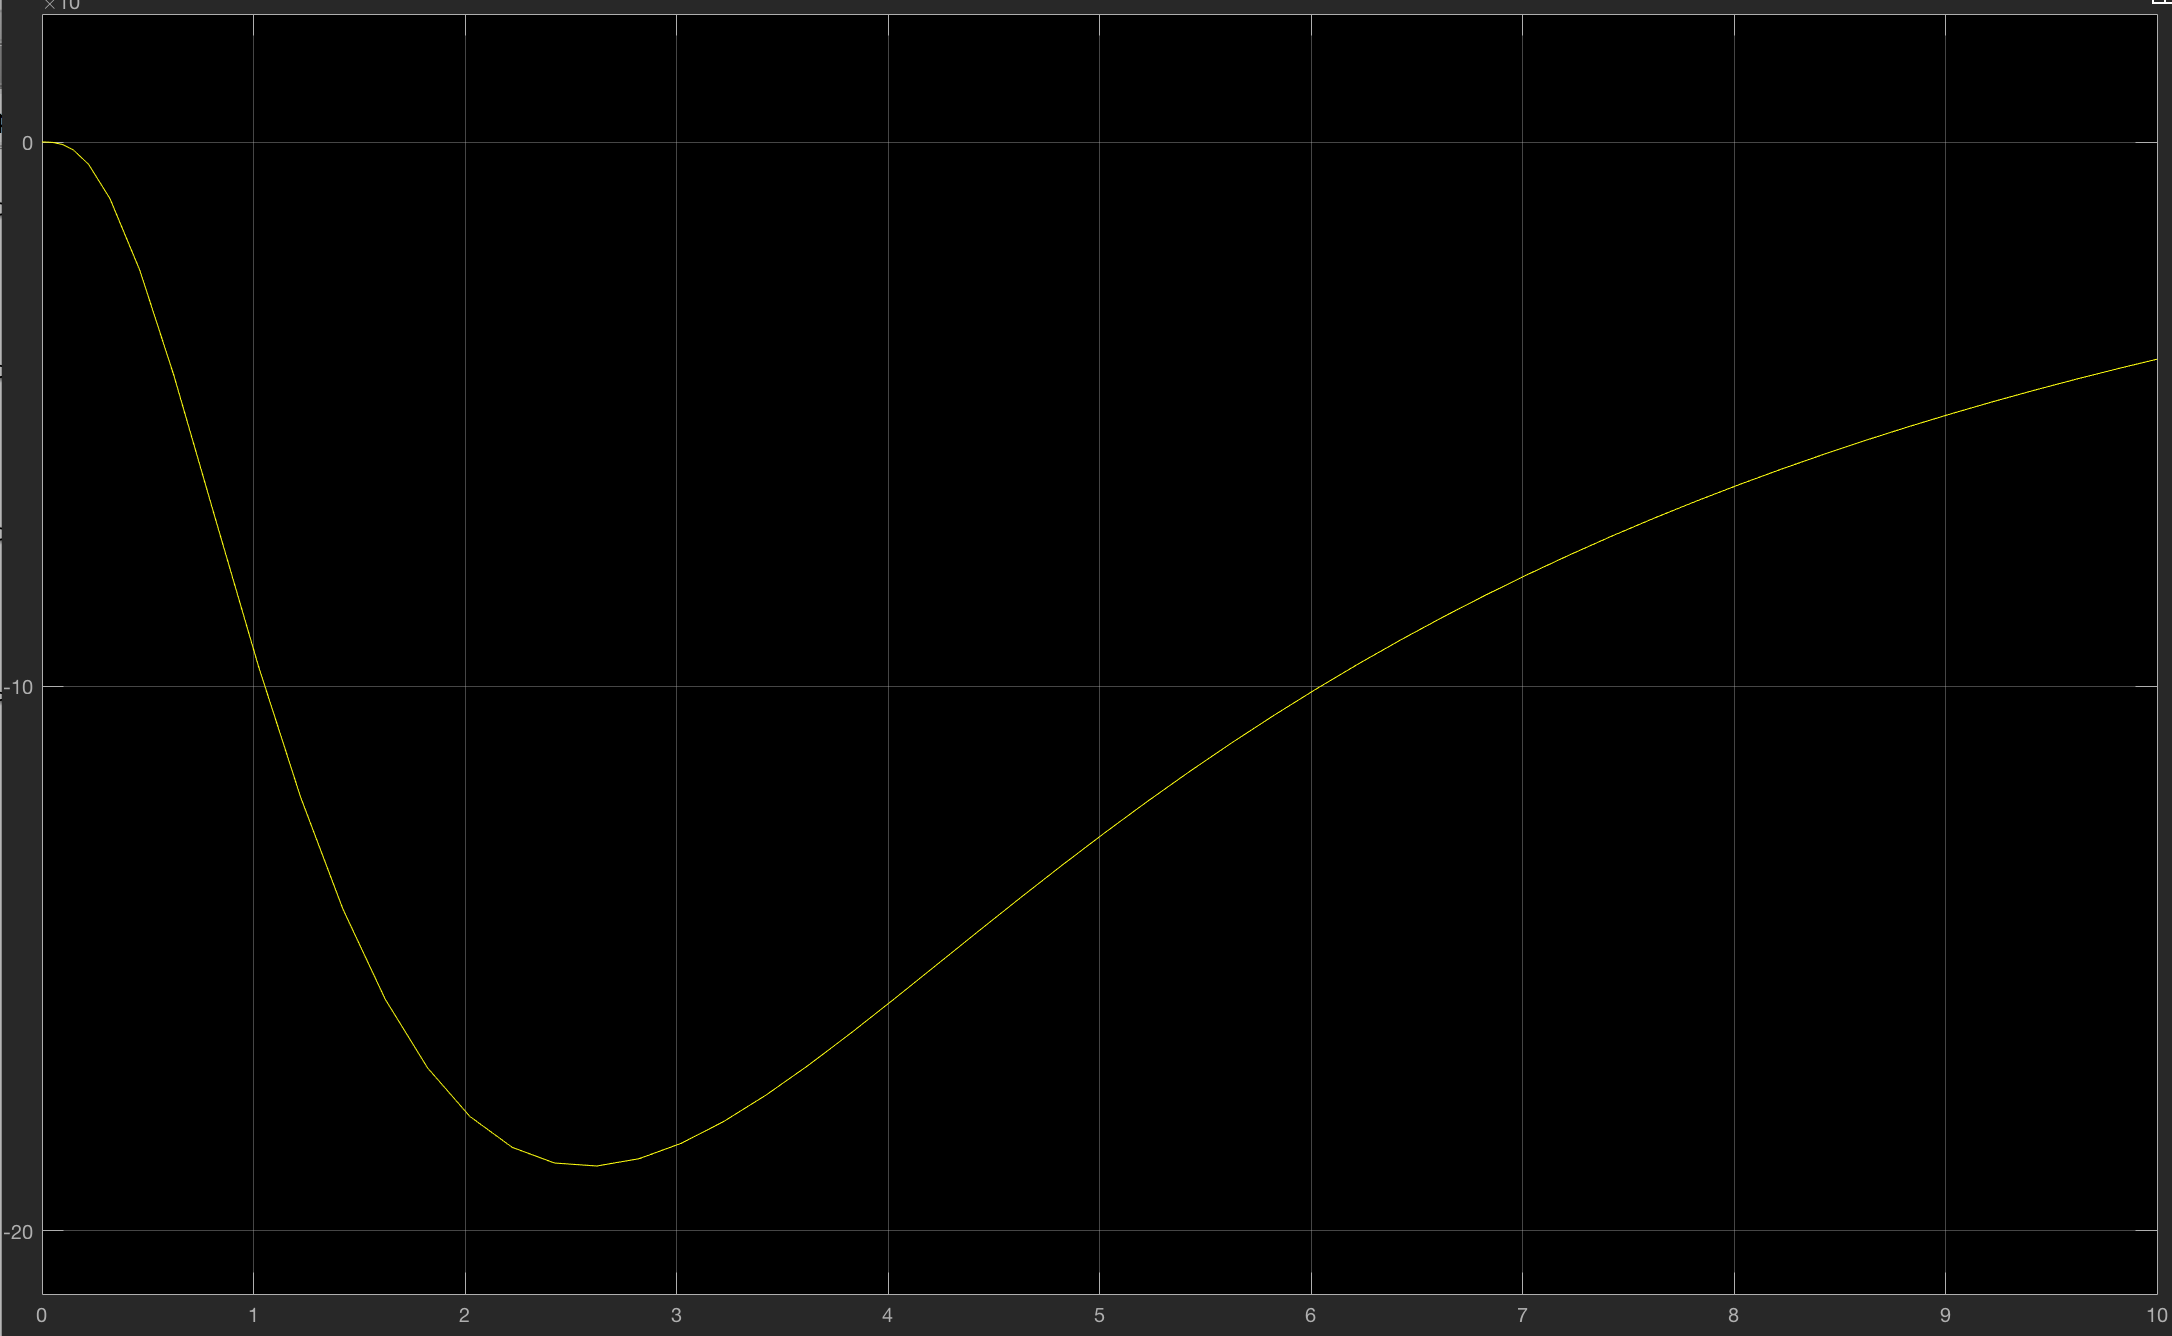
\includegraphics[width=1\textwidth]{images/closedloopGzstep.png}
	\caption{Closed loop response of the Gz output.}
	\label{closedloop4}
\end{figure}

\begin{figure}[H]
  \centering
    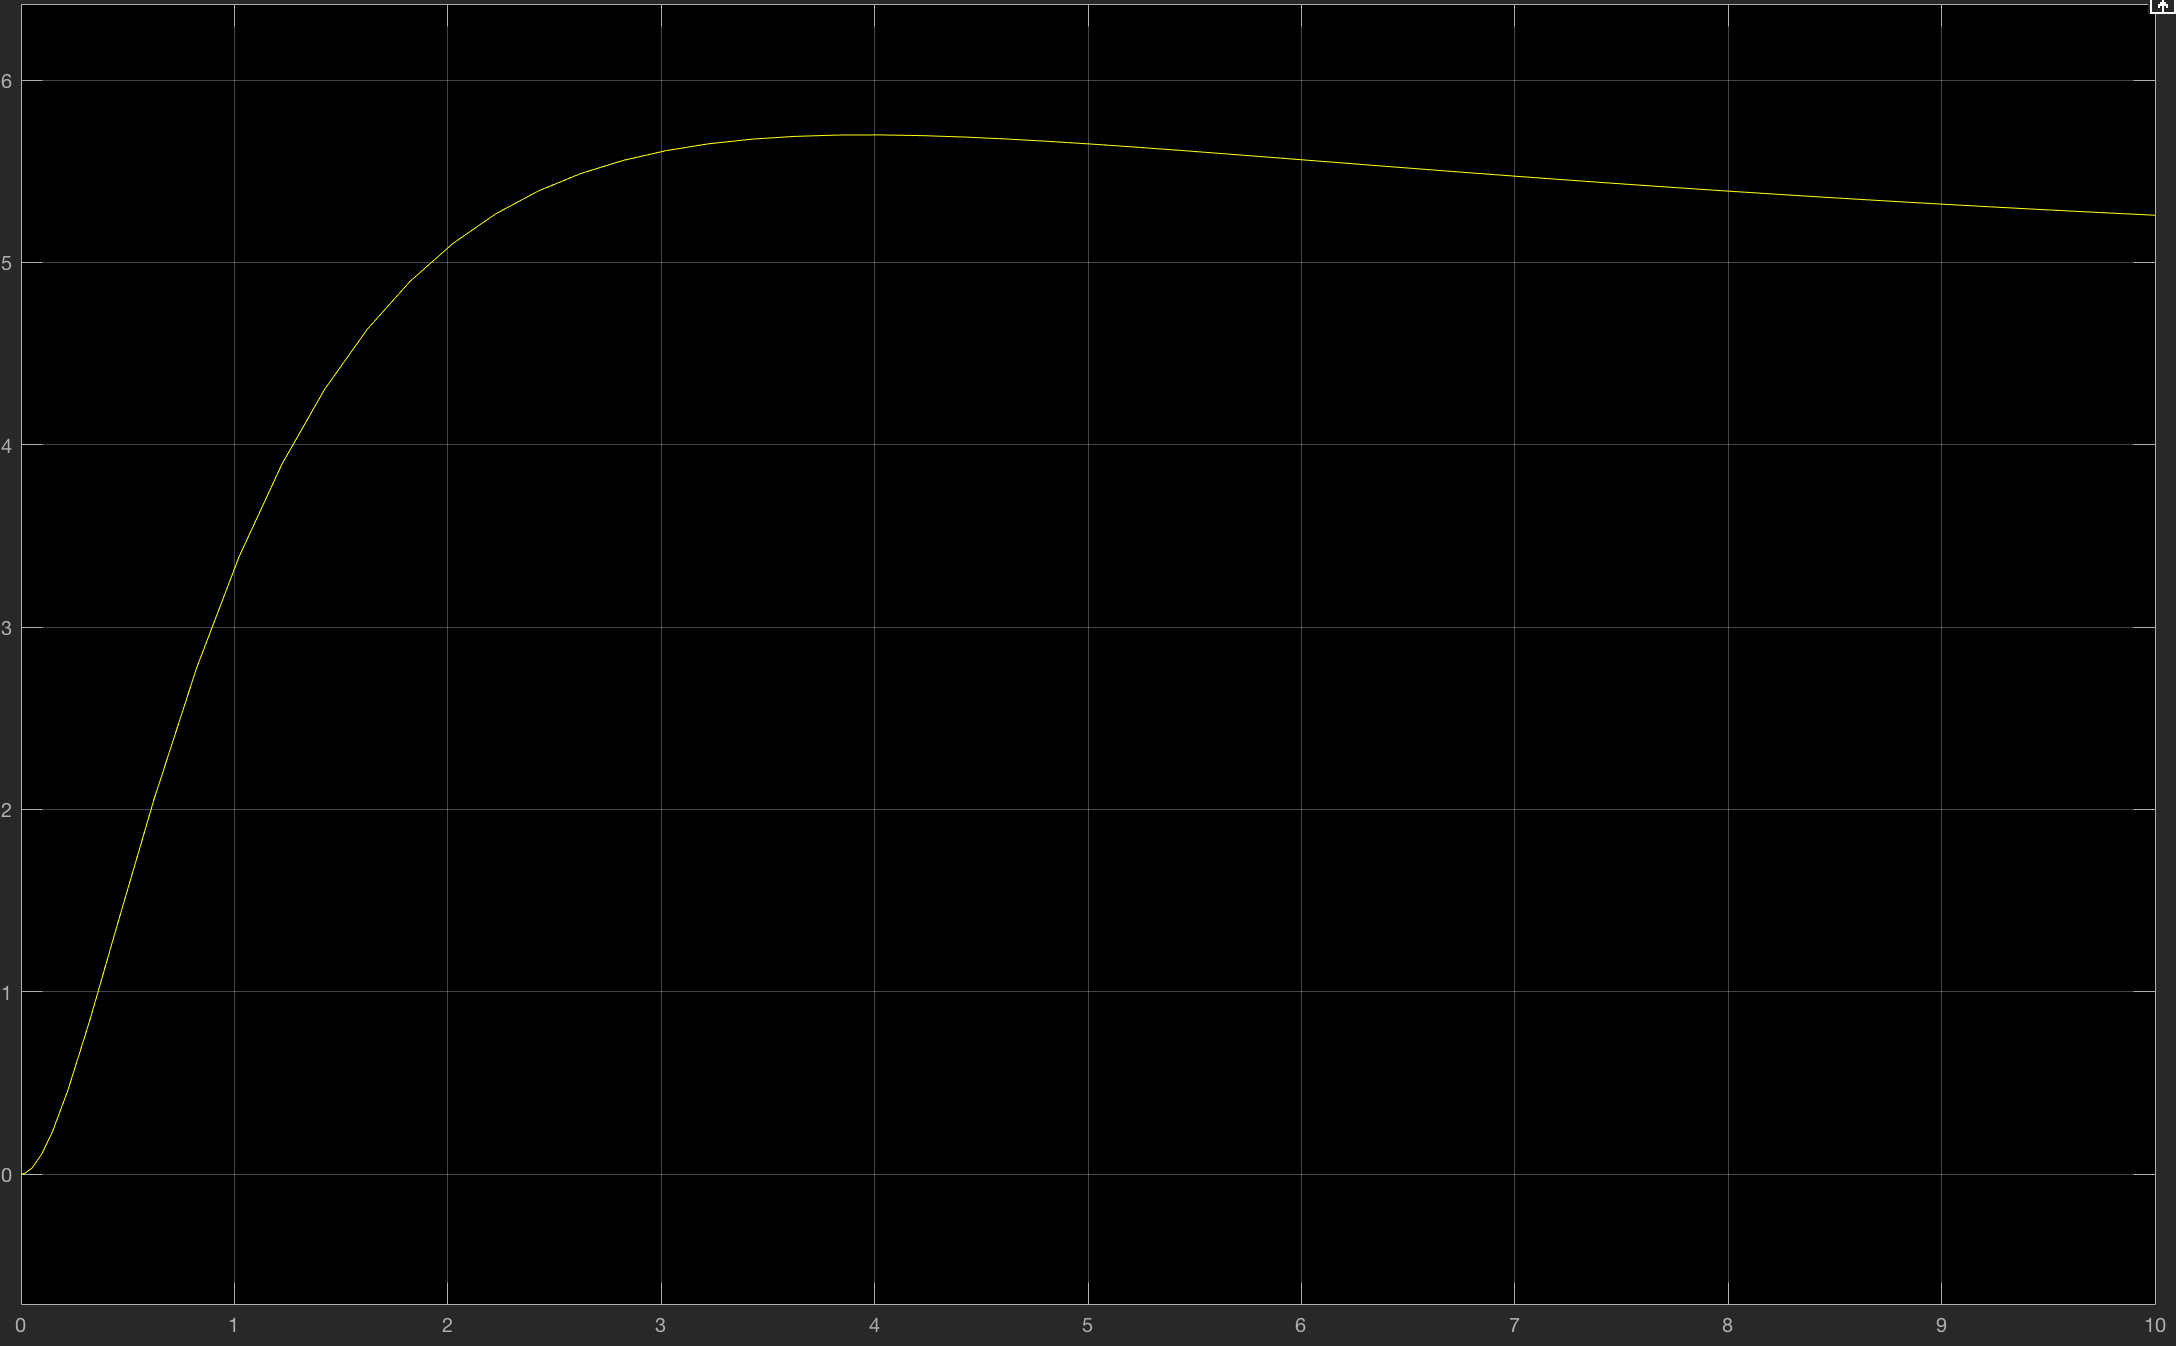
\includegraphics[width=1\textwidth]{images/closedloopNystep.png}
	\caption{Closed loop response of the Ny output.}
	\label{closedloop5}
\end{figure}

The values for each PID used can be seen in Table \ref{PID}.

\begin{table}[H]
\centering
\begin{tabular}{|c|c|c|c|}
\hline
& \textbf{P} & \textbf{I}  & \textbf{D }\\ \hline
\textbf{Gx} & 0.838 & 0.1603 & -0.1766 \\ \hline
\textbf{Gy} & 0.7011 & 0.1341 & -0.1478 \\ \hline
\textbf{Gz} & 0.9804 & 0.1856 & -0.2045 \\ \hline
\textbf{Ny} & -0.17533 & -0.008208 & -0.9197 \\ \hline
\end{tabular}
\caption{PID Controllers values.}
\label{PID}
\end{table}

We can see that the gyroscope outputs tend to go to 0 after the PID implementation and that the Ny output tends to go to the value 5, and that is because the reference for it was set to 5. Ny represents the height that we want our quadcopter to reach, so that makes sense.
